\chapter{Evaluierung}
\label{chp:eval}
  \citet{distrh2} haben gezeigt, dass deren paralleler Ansatz sehr nah an die optimale parallele Effizienz von $\mathcal{O}(\frac{nk}{p})$ herankommt, falls $n$ deutlich größer als $p$ ist.
  Dabei gilt: $n := |\Omega|$ ist die Anzahl Sonnen, $p := |\Proc|$ ist die Anzahl Prozesse und $k := k_0^3$ ist die Anzahl Interpolationspunkte, mit dem Grad der eindimensionalen Lagrange-Polynomen 
  $k_0$. Außerdem sei $m := \frac{n}{p}$ die durchschnittliche Anzahl Elemente pro Prozess.
  
  Im folgenden gilt es diese Argumentation auf den vorliegenden Algorithmus zu übertragen und durch Daten aus praktischen Laufzeitmessungen zu unterstützen. Da unser Algorithmus mit impliziten
  Blockbäumen und \hquad arbeitet, wird die Konstruktion nicht weiter behandelt. Statt dessen konzentrieren wir uns auf eine Abschätzung für die Laufzeit.
  
  \section{Theoretische Abschätzung}
  \label{sec:theo}
  
  Zunächst treffen wir auch für diesen Abschnitt eine Annahme, die bereits bei der Vorstellung des Algorithmus zielführend war:
  \begin{ann} \ \\
  \label{ann:nodes}
    Es existiert $q \in \N$ sodass für $p := \left| \Proc \right|$ gilt:
    \[ p = 2^q \]
  \end{ann}
  
  Zusätzlich zu der sichergestellten vollständigen Binärbaumstruktur benötigt der Clusterbaum für einige Abschätzungen weitere Eigenschaften:
  
  \begin{ann} \ \\
  \label{ann:tree}
    Es existiert eine Konstante $C_{st}$, sodass für alle Teilbäume $T_{sub}$ mit $\tau := root(T_{sub}) \in T_\Omega^{(q)}$ gilt
    \[
     |T_{sub}|\footnotemark \leq C_{st} \frac{n}{kp} \text{ und}
    \]
    \[
     |\tau| \leq C_{st}\frac{n}{p}
    \]
  \end{ann}
  \footnotetext{$|T_{sub}|$ bezeichnet die Anzahl Knoten im Baum}
  
  Diese Annahme wurde durch die Wahl der Abbruchbedingung bei der Konstruktion des Clusterbaumes sichergestellt. Es gilt $|T_{sub}| = \frac{1}{2} \frac{n}{kp}$ (vgl. \autoref{eq:l}),
  da jeder Prozess gerade einen Teilbaum konstruiert, wie er zuvor vom gesamten nicht-parallelisierten Algorithmus vorgenommen wurde (vgl. letzter Absatz in \autoref{sec:data}). Zwar lässt sich die
  Anzahl Elemente der Cluster $\tau \in T_\Omega^{(q)}$ nicht exakt angeben, da die Unterteilung in Sohncluster nicht nach Kardinalität vorgenommen wird, jedoch beträgt diese im Schnitt gerade 
  $m = \frac{n}{p}$. Die Konstante $C_{st}$ kann also als $\approx 1$ angenommen werden.
  
  Die Methode \code{_setup(Cluster *c, int depth)}, die in unserem Algorithmus die Verteilung der Cluster auf Prozesse vornimmt, gewährleistet folgende Eigenschaften:
  
  \begin{bem}
    (Zuständigkeiten)\\
    Für den verteilten Clusterbaum $T_\Omega$ gelten folgende Eigenschaften:
    \begin{equation}
      \text{Für } \tau \in T_\Omega^{(\geq q)} \text{ existiert genau ein } P \in \Proc \text{ mit } \tau.\tcode{activ} = id_P.
    \end{equation}
    \begin{equation}
      \text{Jeder Prozess } P \in \Proc \text{ berechnet auf jeder Ebene } T_\Omega^{(q')}, \ q' \in \nullhaken{q-1} \text{ genau eine Transfermatrix.}\label{eq:log}
    \end{equation}

    Aus \autoref{eq:log} folgt direkt mit $q = \log_2 p$ (vgl. \autoref{sec:work}):
    \begin{equation}
      \text{Die Anzahl Transfermatrizen } E_\tau, \ \tau \in T_\Omega^{(\leq q)} \text{ pro Prozess beträgt } q.\tag{\ref{eq:log}'}
    \end{equation}
  \end{bem}

  Da wir einen parallel arbeitenden Algorithmus haben ist es für die Abschätzung des Rechenaufwandes nicht ausreichend die Anzahl an Operationen zu zählen. Da die Prozesse kommunizieren müssen ist 
  regelmäßig eine Synchronisation der Prozesse notwendig. So wird es vorkommen, dass ein Prozess $P_i$ schneller seine Berechnungen durchführt als ein Prozess $P_j$ und dann auf diesen warten muss bevor
  die Kommunikation stattfinden kann. 
  
  Daher verwenden wir einen ähnlichen Ansatz, wie er auch beim BSP-Modell \citep{bsp} verwendet wurde: Die gesamte Berechnung wird in eine Sequenz von $s \in \N_0$ \textit{Superschritten} eingeteilt,
  die jeweils unabhängig von den anderen Prozessen von einem Prozess durchgeführt werden können. Der $i$-te Superschritt startet simultan, sobald alle Prozesse den $(i-1)$-ten Superschritt abgeschlossen
  haben, $i \in \haken{s}$. Als Zeiteinheit verwenden wir die abstrahierte Einheit \textit{Zyklus}. Ein Zyklus sei dabei lang genug um eine arithmetische Operation, einen Speicherzugriff oder eine Sende-
  oder Empfangsoperation für einen \code{double}-Wert durchzuführen.
  
  \begin{lem}
  \label{lem:vorw}
    (Vorwärtstransformation)\\
    Die parallele Vorwärtstransformation benötigt $\mathcal{O}(\frac{nk}{p}+k^2log_2p)$ Zyklen.
  \end{lem}
  
  \textit{Beweis:} 
  Die gesamte Vorwärtstransformation kann in einem Superschritt abgehandelt werden, da keinerlei Kommunikation notwendig ist. 
  
  Zunächst werden alle aktiven Cluster ausgewertet. Seien also $P \in \Proc$ und $T_\Omega^P$ der aktive Teilbaum dieses Prozesses. Für ein Blattcluster $\sigma \in \mathcal{L}(T_\Omega^P)$ müssen 
  für alle $k$ Ersatzmassen $|\sigma|$ Berechnungen durchgeführt werden.  
  Dann gilt  mit \hyperref[ann:tree]{Annahme }\ref{ann:tree}, dass insgesamt
  \begin{align*}
    \sum_{\sigma \in \mathcal{L}(T_\Omega^P)} k|\sigma| &= k\sum_{\sigma \in \mathcal{L}(T_\Omega^P)} |\sigma| \approx k m\\
    &\leq C_{st}\frac{nk}{p}
  \end{align*}
  Operationen ausgeführt werden müssen.
  
  Für Nicht-Blattcluster $\sigma \in T_\Omega^P \backslash mathcal{L}(T_\Omega^P)$ sind für die $k$ Ersatzmassen und beide Sohncluster wiederum $k$ Auswertungen notwendig. Damit folgt, dass weitere
  \begin{align*}
    &\sum_{\sigma \in T_\Omega^P \backslash \mathcal{L}(T_\Omega^P)} \ \ \sum_{\tilde \sigma \in sons(\sigma)} 2k^2 \leq \sum_{\tilde \sigma \in T_\Omega^P} 2k^2\\
    &= 2k^2 |T_\Omega^P| \leq 2k^2 C_{st} \frac{n}{kp} = 2C_{st}\frac{nk}{p}
  \end{align*}
  Operationen ausgeführt werden müssen.
  
  Für die Ebenen $T_\Omega^{(<q)}$ werden nun jeweils die $k$ Ersatzmassen aus den $k$ Ersatzmassen eines Sohnclusters berechnet. Da es gerade $q = log_2(p)$ Ebenen gibt führt dies insgesamt zu obiger
  Abschätzung. \qed
  
  \begin{lem}
  \label{lem:ruckw}
    (Rückwärtstransformation)\\
    Die parallele Rückwärtstransformation benötigt $\mathcal{O}(\frac{nk}{p}+k^2log_2p)$ Zyklen.
  \end{lem}
  
  \textit{Beweis:}
  Der Beweis läuft analog zu dem von \autoref{lem:vorw}, die Berechnung verläuft lediglich von der Wurzel zu den Blättern statt wie bei der Vorwärtstransformation umgekehrt. \qed
  
  \begin{lem}
  \label{lem:koppl}
    (Kopplungsmatrizen und Nahfeld)
    Die Auswertung der Kopplungs- und Nahfeldmatrizen benötigt $\mathcal{O}(\frac{nk}{p} + k^2 log_2p)$ Zyklen.
  \end{lem}

  \textit{Beweis:}
  Von \citet{distrh2} wurde bewiesen, dass der Speicherbedarf für Nah- und Fernfeldmatrizen $\mathcal{O}(\frac{nk}{p} + k^2 log_2p)$ beträgt. Da der Algorithmus für jedes Element der Matrizen $S_b$ und
  $N_b$ nicht mehr als zwei Auswertungen vornimmt, liegt auch die benötigte Anzahl Zyklen in $\mathcal{O}(\frac{nk}{p} + k^2 log_2p)$. Auch in diesem Schritt ist keine Kommunikation notwendig, sodass 
  auch diese Auswertung in einem Superschritt stattfinden kann. \qed
  
  Bleibt noch die Kommunikation. Diese gliedert sich in zwei Superschritte: Das Vorbereiten mit dem anschließenden Senden der Daten und das Empfangen der Daten. 
  
  \begin{lem}
    (Kommunikation)
    Die Kommunikation benötigt $\mathcal{O}(\frac{nk}{p} + k^2 log_2p)$ Zyklen.
  \end{lem}

  \textit{Beweis:}
  Da die Vorbereitung der Kommunikation nach der selben Struktur wie die Auswertung der Kopplungs- und Nahfeldmatrizen arbeitet, fallen dafür ebenfalls $\mathcal{O}(\frac{nk}{p} + k^2 log_2p)$ Zyklen 
  an. Da ebenso viele Elemente gesendet und empfangen werden müssen liegt der Gesamtaufwand für die Kommunikation in eben dieser Komplexitätsklasse. \qed
  
  Für jeden Superschritt wurde also gezeigt, dass dieser $\mathcal{O}(\frac{nk}{p} + k^2 log_2p)$ Zyklen benötigt. Damit folgt für den gesamten Algorithmus:
  
  \begin{thm}
    Die Berechnung des Algorithmus benötigt $\mathcal{O}(\frac{nk}{p} + k^2 log_2p)$ Zyklen.
  \end{thm}
  
  \citet{distrh2} merken noch an, dass  für genügend große Probleme, also $n \geq k^2 log_2p$, die optimale Komplexitätsordnung von $\mathcal{O}(\frac{nk}{p})$ erreicht wird.
  
  \section{Laufzeitmessung}
  \label{sec:lauf}
  Die theoretischen Argumente des letzten Abschnitts wollen wir nun durch die Messung von Laufzeitdaten des Algorithmus untermauern.
  
  Um diese Daten zu sammeln, wurde das vorliegende auf dem NEC HPC-Linux-Cluster der CAU Kiel ausgeführt. Jeder Knoten dieses Clusters ist mit 192 GB Arbeitsspeicher und zwei Intel Xeon Gold 
  6130 bestückt, die einen Kerntakt von 2,1 GHz aufweisen. Verbunden sind die Knoten über EDR infiniband. Als Compiler wurden der Intel-C-Compiler 17.0.4 sowie der Intel-MPI-Compiler 17.0.4 verwendet.
  
  Es wurden unterschiedliche Testreihen durchgeführt, bei denen entweder die Anzahl Prozesse oder die Anzahl Sonnen variiert wurde, um beide Ansätze unabhängig voneinander testen zu können.
  Alle Tests wurden mit Lagrange-Polynomen von Grad $3$ in jeder Richtung approximiert, was zu $3^3 = 27$ Interpolationspunkten führt. Außerdem wurde jeder Testlauf 10 Mal wiederholt und immer 
  vollständige Knoten im Clustersystem angefordert, um stabile Daten zu ermitteln.
  
  \subsubsection{Approximation}
  \begin{figure}[t]%
  \centering
  \begin{subfigure}{\textwidth}
    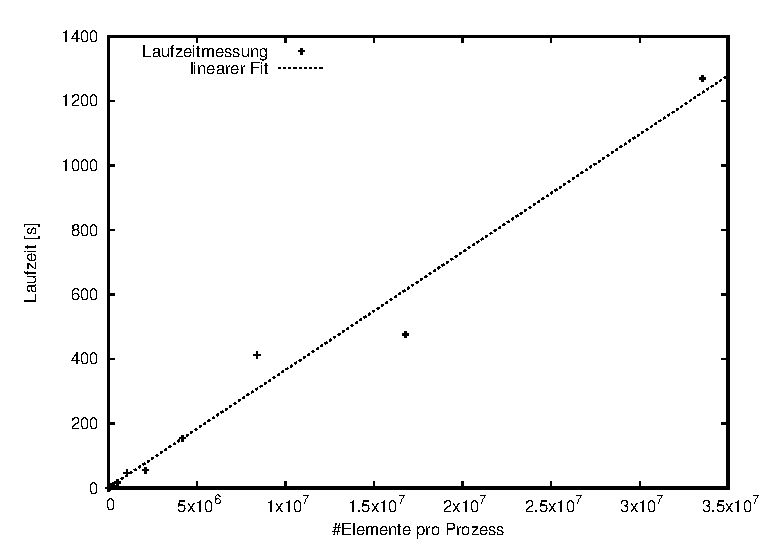
\includegraphics[width=0.8\textwidth]{img/grav1_lin.eps}
    \subcaption{Dieser Testlauf wurde mit $p = 1$ durchgeführt und entspricht damit der nicht-parallelen Variante.}
  \end{subfigure}
  \begin{subfigure}{\textwidth}
    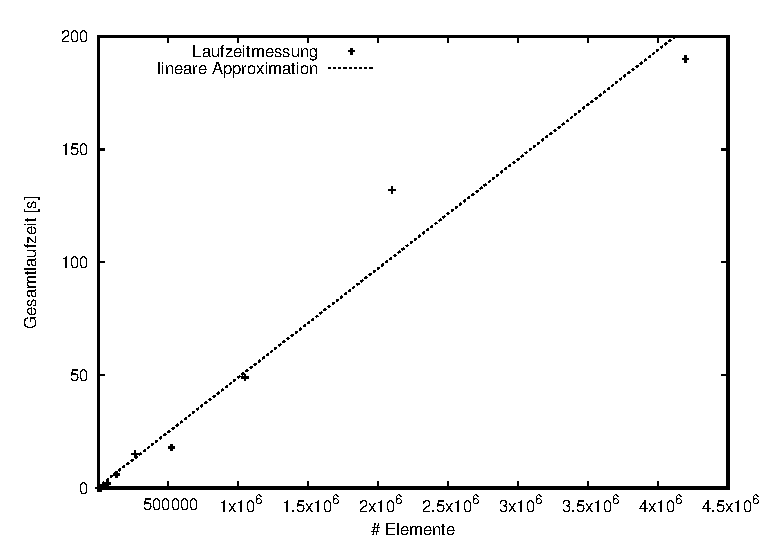
\includegraphics[width=0.8\textwidth]{img/grav_32_lin.eps}
    \subcaption{Dieser Testlauf wurde mit $p = 32$ durchgeführt, genau ein Knoten des Rechenclusters auszulasten.}
  \end{subfigure}
  \caption{In dieser Abbildung ist der Zusammenhang der Laufzeit mit der Anzahl an Elementen pro Prozess dargestellt.}
  \label{fig:1-32x}
\end{figure}
  \begin{table}[t]
 \begin{subtable}{0.45\textwidth}
  \begin{tabular}{c c c}
    \ \ \ \ 
    &
    \begin{tabular}{|P{2cm}|P{2cm}|}
      \hline
      \#Elemente \newline pro Prozess & Laufzeit [s] \\
      \hline
      $2^{10}$ & 0,008324 \\
      $2^{11}$ & 0,02569 \\
      $2^{12}$ & 0,04406 \\
      $2^{13}$ & 0,1348 \\
      $2^{14}$ & 0,503 \\
      $2^{15}$ & 0,6866 \\
      $2^{16}$ & 1,905 \\
      $2^{17}$ & 5,271 \\
      $2^{18}$ & 6,454 \\
      $2^{19}$ & 17,52 \\
      $2^{20}$ & 46,63 \\
      $2^{21}$ & 55,57 \\
      $2^{22}$ & 154,5 \\
      $2^{23}$ & 413,1 \\
      $2^{24}$ & 476 \\
      $2^{25}$ & 1270 \\
      \hline
    \end{tabular}
    &
    \ \ \ \ 
  \end{tabular}
 \subcaption{Dieser Testlauf wurde mit $p = 1$ durchgeführt und entspricht damit der nicht-parallelen Variante.}
 \end{subtable} \ \ 
 \begin{subtable}{0.45\textwidth}
  \begin{tabular}{c c c}
    \ \ \ \ 
    &
    \begin{tabular}{|P{2cm}|P{2cm}|}
      \hline
      \#Elemente \newline pro Pozess & Laufzeit [s] \\
      \hline
      $2^{10}$ & 0,02877 \\
      $2^{11}$ & 0,06701 \\
      $2^{12}$ & 0,1962 \\
      $2^{13}$ & 0,3097 \\
      $2^{14}$ & 0,7803 \\
      $2^{15}$ & 2,402 \\
      $2^{16}$ & 3,288 \\
      $2^{17}$ & 8,54 \\
      $2^{18}$ & 19,9 \\
      $2^{19}$ & 27,01 \\
      $2^{20}$ & 65,41 \\
      $2^{21}$ & 170 \\
      $2^{22}$ & 239,1 \\
      $2^{23}$ & 580,4\\
      & \\
      & \\
      \hline
    \end{tabular}
  \end{tabular}
 \subcaption{Dieser Testlauf wurde mit $p = 32$ durchgeführt, um genau ein Knoten des Rechenclusters auszulasten.}
 \end{subtable}
\caption{In dieser Tabelle sind die Laufzeitmessungen der ersten beiden Testläufe aufgeführt.}
\label{tab:1-32x}
\end{table}

  \begin{table}[b]
    \begin{tabular}{|l|c c c c c c c|}
%     \hline
%     $k_0$ & 1 & 2 & 3 & 4 & 5 & 6 & 7\\
    \hline
    $k$ & 1 & 8 & 27 & 64 & 125 & 216 & 343\\
    \hline
    Fehler & $5,12e^{-2}$ & $8,58e^{-3}$ & $8,11e^{-4}$ & $9,38e^{-5}$ & $9,67e^{-6}$ & $1,21e^{-6}$ & $7,4e^{-15}$\\
    \hline
    Laufzeit [s] & 0,0486 & 0,0967 & 0,259 & 0,454 & 0,864 & 1,09 & 1,3\\
    \hline
    \end{tabular}
    \caption{Die Tabelle zeigt den Approximationsfehler und die Laufzeit in Abhängigkeit zur Interpolationsordnung.\TODO{besser erklären}}
    \label{tab:error}
  \end{table}
  
  In den ersten beiden Testreihen wurde die Anzahl Sonnen pro Prozess bei konstanter Anzahl Prozesse variiert. Die Messergebnisse sind in \autoref{tab:1-32x} sowie in \autoref{fig:1-32x} 
  aufgeführt.
  
  Abbildung beziehungsweise Tabelle \textbf{(a)} bezieht sich jeweils auf die Testreihe mit einem Prozess, \textbf{(b)} auf die Testreihe mit 32 Prozessen. Trotz einiger Schwankungen, deren Herkunft
  nicht festgestellt werden konnte, ist der lineare Zuwachs gut zu erkennen. Bei der eingezeichneten Geraden handelt es sich um eine von gnuplot berechnete Regressionsgrade. Der Testlauf mit $32$ 
  Prozessen zeigt eine etwas stärkere Steigung, die vermutlich auf den erhöhten Kommunikationsaufwand zurückzuführen ist. Dennoch ist zu erkennen, dass die Approximation durch Interpolation und die 
  Nutzung der $\mathcal{H}^2$-Struktur den theoretischen Berechnungen auch in reellen Anwendungen gerecht wird und die Komplexität von $\mathcal{O}(n^2)$ auf $\mathcal{O}(k n)$ senken kann. Da $k$ 
  wesentlich kleiner als $n$ ist, ist damit viel gewonnen.
  
  Um diese $\mathcal{H}^2$-Struktur nutzen zu können hatten wir die eigentliche Kernfunktion durch Interpolation approximiert. Zwar haben wir über eine Zulässigkeitsbedingung sichergestellt, dass die 
  Ergebnisse ``vernünftig'' sind und Beweise angeführt, nach denen diese Approximation mit steigender Ordnung exponentiell gegen die eigentliche Kernfunktion konvergiert, aber wie ungenau wird die
  Berechnung durch die Approximation? Dazu wurden im kleineren Maßstab\footnote{Ausgeführt auf einem Computer mit 16 Gb Arbeitsspeicher und einem Intel Core i7-4710HQ.} einige Testläufe durchgeführt, 
  die ebenfalls sehr stabile Resultate gezeigt haben. Die Ergebnisse sind in \autoref{tab:error} zu finden.
  
  \todo{genauer ausarbeiten!}Wie an den Daten zu erkennen ist, nimmt der Fehler bei jeder Erhöhung der Interpolationsordnung $k_0$ um etwa Faktor $8$ ab. Unsere Approximation konvergiert also wie vorgesehen exponentiell. Natürlich
  dauert die Berechnung für mehr Interpolationspunkte länger. Zu erkennen ist außerdem, dass bei diesem Testlauf bei $k_0=7$ eine Art Plateau erreicht wurde. Weitere Erhöhung hat keine Signifikante
  Änderung der Fehlerwerte mehr ergeben. Dies scheint mit den Ebenen des Clusterbaumes zusammenzuhängen. Wird die Interpolationsordnung gegenüber der Anzahl Sonnen groß genug, werden durch den
  vorliegenden Algorithmus zu wenig Ebenen im Clusterbaum erzeugt, sodass entsprechend wenig zulässige Blöcke gefunden werden können. Dies erklärt sowohl den plötzlichen Anstieg an Genauigkeit und
  die anschließende Stagnation.
  
  \subsubsection{Parallelität}
  \begin{figure}
  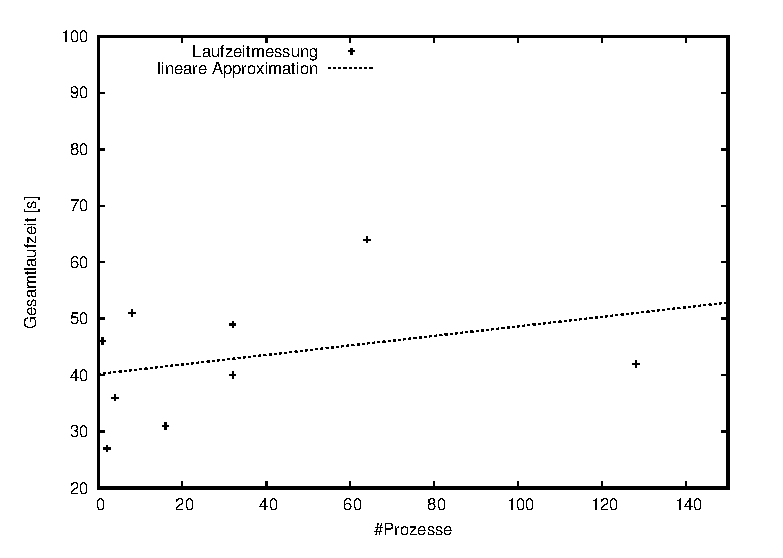
\includegraphics{img/grav_X20_lin.eps}
  \caption{Dieses Diagramm zeigt den Anstieg der Laufzeit in Abhängigkeit zur Anzahl Prozesse.}
  \label{fig:x20}
\end{figure}

\begin{table}[b]
  \begin{tabular}{|c|c|}
    \hline
    \#Prozesse & Laufzeit [s] \\
    \hline
    1 & 46,54 \\
    2 & 27,73 \\
    4 & 36,94 \\
    8 & 51,94 \\
    16 & 31,29 \\
    32\footnote{Die 32 Prozesse befanden sich auf einem Knoten des Clustersystems.} & 49,42 \\
    32\footnote{Die 32 Prozesse verteilten sich zu je 16 auf zwei Knoten des Clustersystems.} & 40,82 \\
    64 & 64,96 \\
    128 & 42,27 \\
    \hline
  \end{tabular}
  \caption{Tabelle der gemessenen Laufzeitdaten in Abhängigkeit zur Anzahl Prozesse.}
  \label{tab:x20}
\end{table}


  Bereits durch die höhere Steigung der Graden in \autoref{fig:1-32x}.\textbf{(b)} gegenüber der in \textbf{(a)} lässt sich erahnen, dass durch die Kommunikation bei der Parallelisierung ein gewisser
  Overhead verursacht wird. Um dies genauer zu untersuchen wurde die Anzahl Sonnen pro Prozess\footnote{Mit einer Verdoppelung der Prozessanzahl geht also auch eine Verdopplung der Anzahl Sonnen 
  einher.} auf $m = 2^{20}$ fixiert und die Anzahl Prozesse variiert.  Die Messdaten sind in \autoref{tab:x20} und \autoref{fig:x20} zu finden. 
  
  Die Daten unterliegen leider recht großen Schwankungen. Woher diese Schwankungen stammen muss an anderer Stelle genauer untersucht werden, da es den Umfang und die Zielsetzung dieser Arbeit 
  übersteigt. Allerdings waren diese Ergebnisse in sich sehr stabil. Auch mehrfache Wiederholungen der einzelnen Testläufe haben immer bis auf wenige Zehntelsekunden die selbe Zeit benötigt. 
   Trotzdem scheint mir, dass die errechnete Regressionsgrade die allgemeine Tendenz der Laufzeit einigermaßen akkurat wiedergibt.
  
  Ein gewisser Anstieg der Laufzeit ist zu erwarten, da der Kommunikationsaufwand steigt. Insgesamt zeigt sich aber die fast optimale Ausnutzung der Parallelität.
  
  Ein interessanter Effekt kann an den mit Fußnoten \textit{a} und \textit{b} gekennzeichneten Testläufen beobachtet werden. Während bei \textit{a} alle Prozesse auf einem Knoten gearbeitet haben, 
  wurden diese für den Testlauf \textit{b} auf zwei Knoten verteilt. Eine an sich naheliegende Vermutung wäre, dass die Testparameter für \textit{a} bessere Laufzeiten ergeben müssten,
  da die Kommunikation auf einem Rechner und ohne Netzwerkbeteiligung stattfinden kann. In der Realität hat sich aber gezeigt, dass es gerade umgekehrt ist. Vermutlich behindern sich die vielen 
  Speicherzugriffe bei dem Testlauf auf einem Knoten so stark, dass es effektiver ist einen Teil der Kommunikation über das Netzwerk zu führen. Auch dieser Effekt müsste aber an anderer Stelle 
  genauer untersucht werden.
  
  \clearpage
  
  \subsubsection{Speicherbedarf der Kommunikation}
  Bei all den positiven Eigenschaften sei auch auf einen Nachteil des vorgestellten Algorithmus hingewiesen: Die verwendete Kommunikation benötigt viel unnötigen Speicher. Mein Hauptaugenmerk lag
  darauf, die Kommunikation so einfach wie möglich zu gestalten, um die Laufzeit möglichst gering zu halten. Da die \code{MPI_Alltoallv(..)}-Methode exakt das benötigte Kommunikationsmuster liefert
  und davon auszugehen ist, dass bei der Implementierung dieser Methode mehr Zeit und Know-How eingeflossen ist, als ich im Rahmen dieser Arbeit hätte investieren können, habe ich mich dazu entschieden
  diese Methode zu nutzen. Die dafür notwendigen Puffer waren recht schnell konstruiert und wurden von mir zunächst nicht weiter beachtet. 
  
  Es hat sich aber gezeigt, dass bei 32 Prozessen auf einem Knoten mit $2^{22}$ Sonnen pro Prozess bereits $182$ GB Arbeitsspeicher benötigt werden. Das sind $5,68$ GB pro Prozess. Vergleicht man dies
  mit dem Testlauf mit nur einem Prozess, der lediglich $52.37$ MB Hauptspeicher belegt, ist schnell einzusehen, dass die Kommunikation mit derart riesigem Pufferbedarf nicht tragbar ist.
  \TODO{ausarbeiten!}
  
  Ganz ohne Puffer wird die Kommunikation nie auskommen. Es wäre aber möglich die Kommunikation durch nicht-blockierende Methoden derart zu verteilen, dass keinerlei Sendepuffer und lediglich 
  Empfangspuffer für nicht-zulässige Blöcke benötigt würden. Dieser Ansatz ähnelt stärker dem von \citet{distrh2} vorgestellten Algorithmus, jedoch wäre weiterhin keine Kommunikation für Vorwärts- und 
  Rückwärtstransformation notwendig. Eine genaue Ausarbeitung eines solchen Ansatzes muss leider aus Zeit- und Umfangsgründen an anderer Stelle fortgesetzt werden.
  
  